\documentclass[12pt]{article}

\usepackage{sbc-template}

\usepackage{graphicx,url}

%\usepackage[brazil]{babel}   
\usepackage[utf8]{inputenc}  
     
\sloppy

\title{NOSQL - Armazenamento e Recuperação de dados não-relacional}

\author{Bruno Santos de Lima\inst{1}, Leandro Ungari Cayres\inst{1} }


\address{Faculdade de Ciências e Tecnologia\\
  Universidade Estadual Paulista \\
  "Júlio de Mesquita Filho" \\
  Caixa Postal 19060-900  -- Presidente Prudente -- SP -- Brasil
  \email{brunoslima4@gmail.com, leandroungari@gmail.com}
}

\begin{document} 

\maketitle

\begin{abstract}
Traduzir o resumo...
\end{abstract}
     
\begin{resumo} 
Fazer... (última coisa)
\end{resumo}


\section{Introdução}
\label{sec:intro}
Irrefutavelmente, é possível notar o crescimento da tecnologia com isso o número de dispositivos eletrônicos, sejam eles supercomputadores, computadores desktop ou aplicações moveis, vem aumento em grandes proporções tornando-se presentes nas mais variadas situações do dia a dia, cada qual buscando manipulando diversos dados referentes ao contexto em que eles são aplicados, seja no âmbito empresarial, hospitalar, juridico, academico e diversos outros setores.

Com as diversas aplicações e diversos dispositivos atuando diariamente na vida da sociedade no que diz respeito a manipulação de dados, surge a necessidade de realizar inicialmente o armazenamento desses dados afim de poder manipula-los de forma eficiente e segura para abstrair informações relevantes sobre determinado contexto onde esses dados estão inseridos e com isso facilitar, ajudando a sociedade a utilizar essas informações para realizar algumas atividades diarias, o responsavel por realizar esse armazenamento e conseguentemente a manipulação desses dados é o chamado Banco de dados.

Quando o assunto Banco de dados é abordado logo é pensado como os dados não armazenados e manipulados? para isso é seguido um modelo, de certa forma uma padronização, para responder esta pergunta, o modelo mais conhecido e utilizado em larga escala por Sistemas Gerenciadores de Banco de Dados (SGBD's) é denominado modelo relacional \cite{codd:1970} criado por Edgar Frank Codd em 1970, o modelo relacional substituiu o modelo anterior chamado de modelo hierarquico tornando-se um padrão referencia para este quesito, sendo utilizado pela grande maioria dos SGBD's, onde podemos citar por exemplo os mais conhecidos atualmente: MySQL, Oracle, SQL Server e PostgreSQL. \cite{brito2010bancos}

Este artigo esta organizado como segue: na seção \ref{sec:nosql}.....

%melhorar e acrescentar bem mais....

\section{NOSQL} 
\label{sec:nosql}

O decorrer do tempo foi pensando em modelagens alternativas ao tão utilizado modelo relacional, tais pensamentos justificam-se devido a algumas limitações presente no modelo relacional, limitações essas relacionadas a falta de felxibilidade fornecidade pelo modelo.

Os Banco de dados NoSQL fornecem mecanismos de aramzenamento e recuperação de dados que são modelados como não estruturado, diferente da forma disposta por tabelas utilizada pelos Banco de dados Relacionais. \cite{zhaoSchema:2014}

%melhorar a justificativa para buscar um outro modelo...

%falar mais

%Trabalhar aqui!!!!

\subsection{Categorização dos Banco de dados NOSQL}
\label{subsec:categorizacao}

O NOSQL pode ser classificado em cinco categorias \cite{typeNOSQL:2013} sendo elas: Banco de dados de armazenamento chave-valor, Banco de dados orientado por colunas, Banco de dados orientado a documentos, Banco de Dados orientado a grafos e Banco de Dados orientado a objetos.

Em Banco de dados de armazenamento chave-valor os dados tem duas informações associadas a ele, uma sendo a chave e a outra sendo o valor, onde esse valor é literalmente o dado armazenado, como isso seu mecanismo de funcionamento atua de forma similar a um hash, trazendo como um aspecto positivo a rapidez em sua manipulação, não só isso mas também alta concorrência e armazenamento em massa, porem o grande ponto negativo deve-se a falta de uma esquematização o que deixa a visualização da organização desses dados dificultada. \cite{typeNOSQL:2013}

Em Banco de dados orientado por coluna consiste em uma organização onde o dados não são armazenados em linhas mas sim em colunas, ou seja, ocorre uma mudança de orientação agora sendo por atributos, colunas, e não mais por registros, tuplas. Dois exemplos dessa categoria de Banco de dados orientado por colunas é o Cassandra e o BigTable. \cite{brito2010bancos}\cite{surveyNosql:2012}

Em Banco de dados orientado a documentos os dados são armazenados na forma de documentos que tem uma chave unica associada a ele, essa chave é uma string que representa o caminho, ou URI, onde o documento está armazenado, no geral é fonecido uma API ou uma linguagem de consulta para que esses documentos possam ser recuperados rapidamente. \cite{surveyNosql:2012} Uma vantagem relacionado a essa categoria está no aproveitamento de espaço de armazenamento, visto que um documento tem um tamanho necessario para armazenar os dados em que nele estão sem que ocorra desperdicio de espaço, já no modelo relacional os dados são armazenados em tabelas sendo que alguns campos dessa tabela podem ficar vazios disperdiçando espaço, um exemplo de SGBD que utiliza este modelo o MongoDB. Esse modelo deve ser evitado em aplicações que envolvem muitos relacionamentos. \cite{typeNOSQL:2013}

Em Banco de dados orientado a grafos armazenam os dados na forma de um grafo, sendo que cada nó é um objeto e o relacionamento entre esses objetos é expresso pelas arestas que ligam dois nós. Esse tipo de modelo é indicado para redes sociais, sistemas bioinformatica entre outros, pois os nós podem representar por exemplo pessoas ou negocios semelhantes aos objetos utilizados em determinadas linguagens de programação, entretanto apresenta um desvantagem pois é dificil realizar um agrupamento desses dados.\cite{typeNOSQL:2013}\cite{surveyNosql:2012} 

Em Banco de dados orientado a objetos os dados são armazenados na forma de objetos, objetos analogos aos do paradigma de programação orientado a objetos oferecendo recursos como encapsulamento, polimorfismo e herança, cada objeto tem um idenficador unico que representa o objeto unicamente.\cite{typeNOSQL:2013}

\section{Sistemas Gerenciadores de Banco de Dados Não relacionais}

\section{Banco de dados: relacional vs não relacional}

In some conferences, the papers are published on CD-ROM while only the
abstract is published in the printed Proceedings. In this case, authors are
invited to prepare two final versions of the paper. One, complete, to be
published on the CD and the other, containing only the first page, with
abstract and ``resumo'' (for papers in Portuguese).

\section{Armazenamento e recuperação em banco de dados não relacional}

Section titles must be in boldface, 13pt, flush left. There should be an extra
12 pt of space before each title. Section numbering is optional. The first
paragraph of each section should not be indented, while the first lines of
subsequent paragraphs should be indented by 1.27 cm.

\subsection{Subsections}

The subsection titles must be in boldface, 12pt, flush left.

\section{Figures and Captions}\label{sec:figs}


Figure and table captions should be centered if less than one line
(Figure~\ref{fig:exampleFig1}), otherwise justified and indented by 0.8cm on
both margins, as shown in Figure~\ref{fig:exampleFig2}. The caption font must
be Helvetica, 10 point, boldface, with 6 points of space before and after each
caption.

\begin{figure}[ht]
\centering
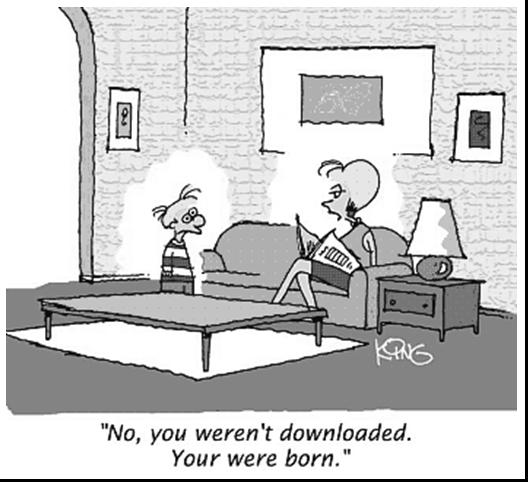
\includegraphics[width=.5\textwidth]{fig1.jpg}
\caption{A typical figure}
\label{fig:exampleFig1}
\end{figure}

\begin{figure}[ht]
\centering
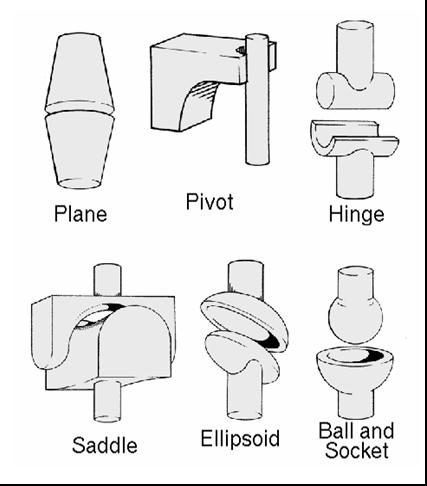
\includegraphics[width=.3\textwidth]{fig2.jpg}
\caption{This figure is an example of a figure caption taking more than one
  line and justified considering margins mentioned in Section~\ref{sec:figs}.}
\label{fig:exampleFig2}
\end{figure}

In tables, try to avoid the use of colored or shaded backgrounds, and avoid
thick, doubled, or unnecessary framing lines. When reporting empirical data,
do not use more decimal digits than warranted by their precision and
reproducibility. Table caption must be placed before the table (see Table 1)
and the font used must also be Helvetica, 10 point, boldface, with 6 points of
space before and after each caption.

\begin{table}[ht]
\centering
\caption{Variables to be considered on the evaluation of interaction
  techniques}
\label{tab:exTable1}
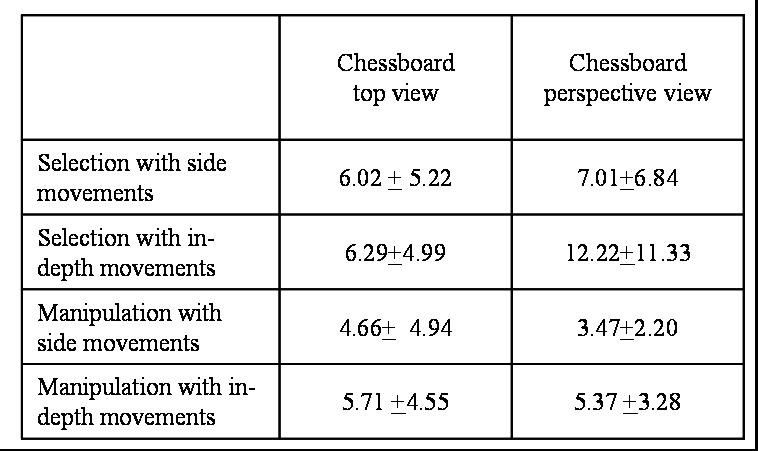
\includegraphics[width=.7\textwidth]{table.jpg}
\end{table}

\section{Conclusão}
\label{sec:conclusao}

All images and illustrations should be in black-and-white, or gray tones,
excepting for the papers that will be electronically available (on CD-ROMs,
internet, etc.). The image resolution on paper should be about 600 dpi for
black-and-white images, and 150-300 dpi for grayscale images.  Do not include
images with excessive resolution, as they may take hours to print, without any
visible difference in the result. 

\bibliographystyle{sbc}
\bibliography{sbc-template}

\end{document}
